%第3章


\section{要求定義}


商品識別システムがどのように機能すべきかという振る舞いと,その外部環境を表すためにユースケース図を作成した.以下に最初に作成した図\ref{usecase1}を載せる.

\begin{figure}[htbp]
\centering
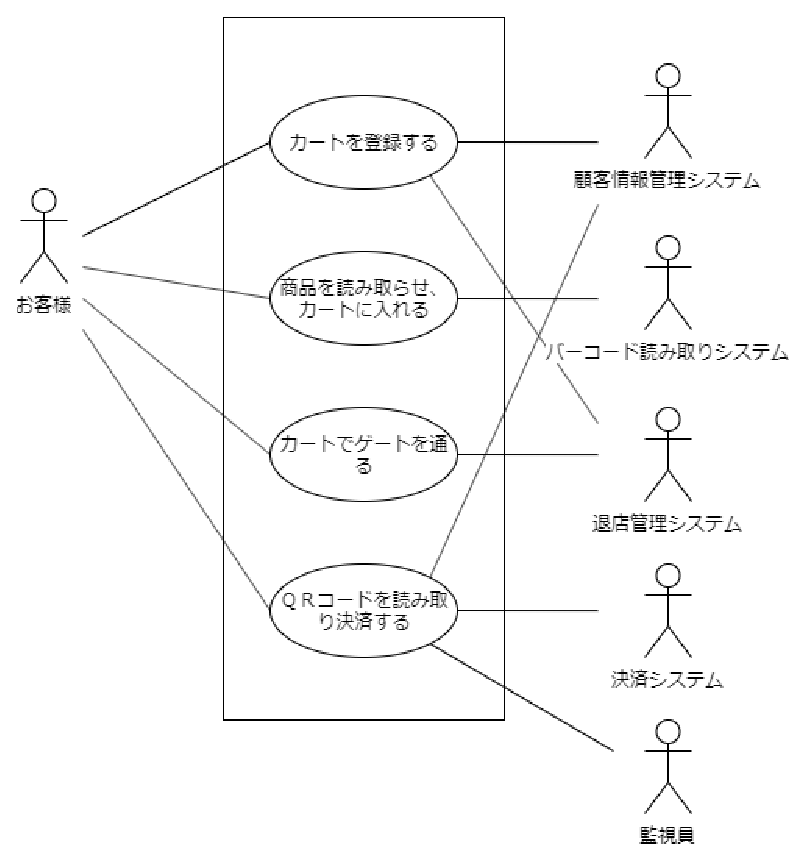
\includegraphics[width = 9cm]{./picture/usecase1.eps}
\caption{ユースケース図(1)}
\label{usecase1}
\end{figure}


図\ref{usecase1}においてユースケースとしてはカートの登録,商品をカートに入れる,カートでゲートを通る,QRコードを読み取り決済するの4つとした.カゴ情報と顧客情報の管理をカートの登録とカートでゲートを通るの2つのユースケースで行おうと設計したが,簡単に決済まで行えるという前提から,ユースケースの数が少ないほうが手順が減り簡単という条件により適すると考え,ユースケースを見直し,全体のユースケース数を削減した.

%退店管理がどうなってたか思い出せないため,usecase2の図はお蔵入り予定
%\begin{figure}[htbp]
%\centering
%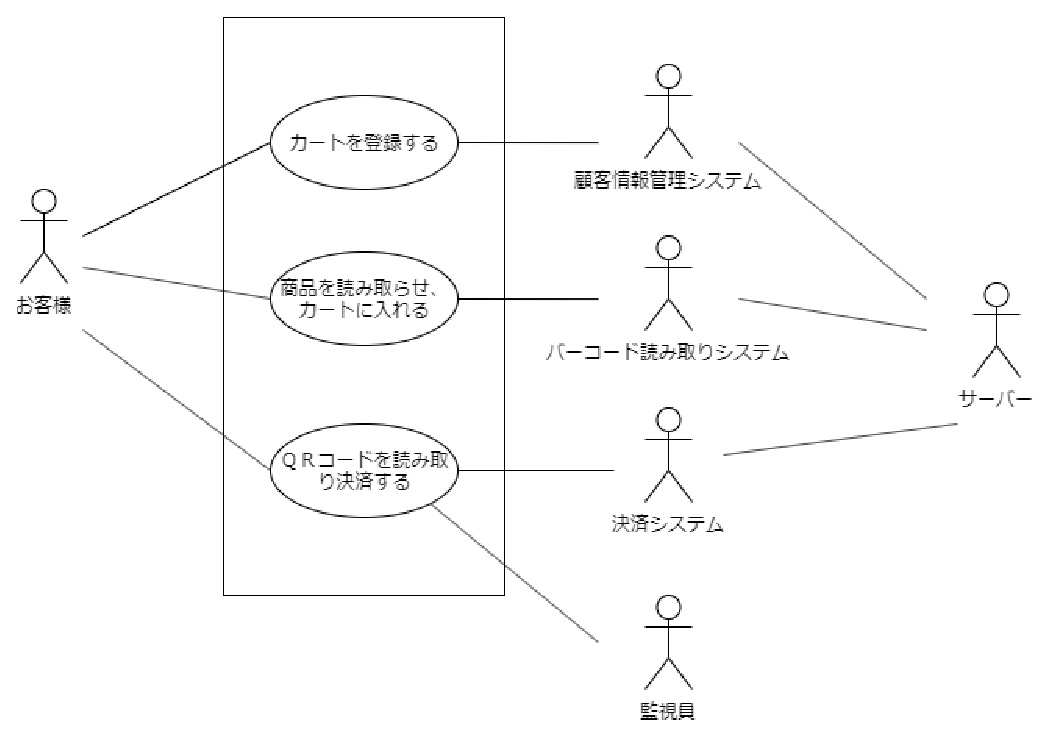
\includegraphics[width = 11cm]{./picture/usecase2.eps}
%\caption{ユースケース図(2)}
%\label{usecase2}
%\end{figure}

ユースケースを見直しユースケースの数を減らしたユースケース図は図\ref{usecase3}に示す.

\begin{figure}[htbp]
\centering
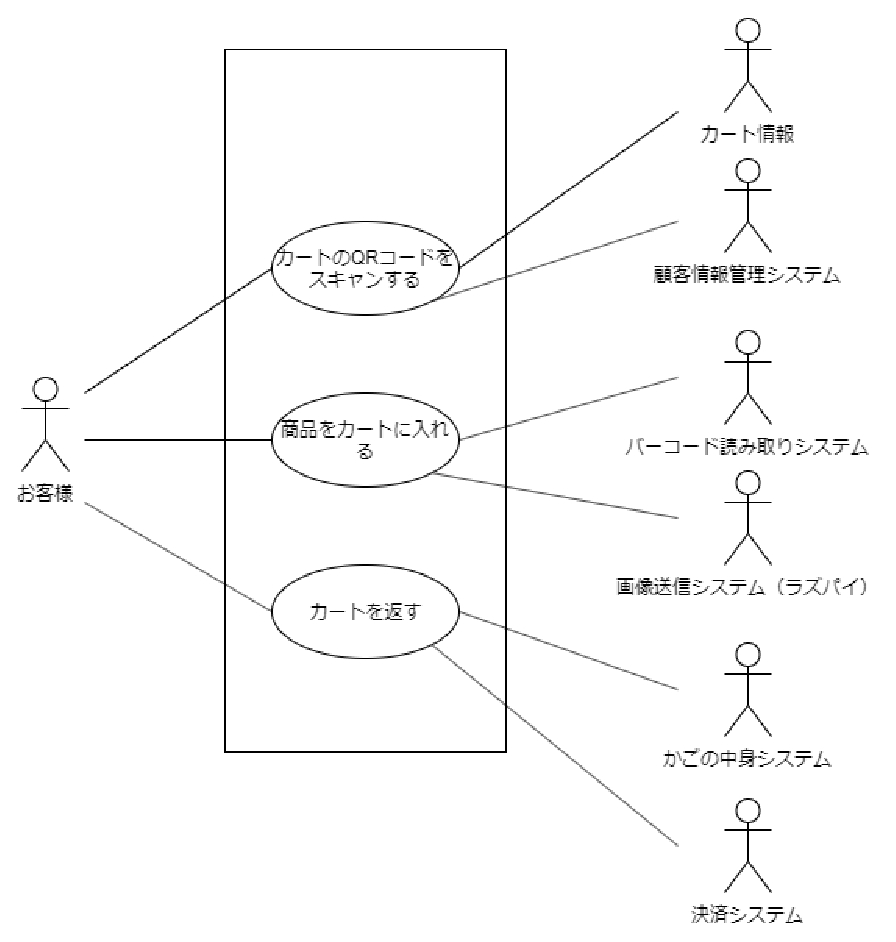
\includegraphics[width = 9cm]{./picture/usecase3.eps}
\caption{ユースケース図(2)}
\label{usecase3}
\end{figure}


図\ref{usecase3}では,QRコードを読み取り決済していた部分を,カートの返却時カゴの情報と顧客情報と結び付け,自動的に決済を行う仕様としたためユースケースが3つとなりより簡素化された.

ここで,問題となったのはカゴ情報と顧客情報を結びつけたり,解除したりする方法である.QRコードを用いる案と,ICタグを用いる案の2つの案について検討すべく,それぞれの案についてユースケース図を作成した.


\begin{figure}[htbp]
\centering
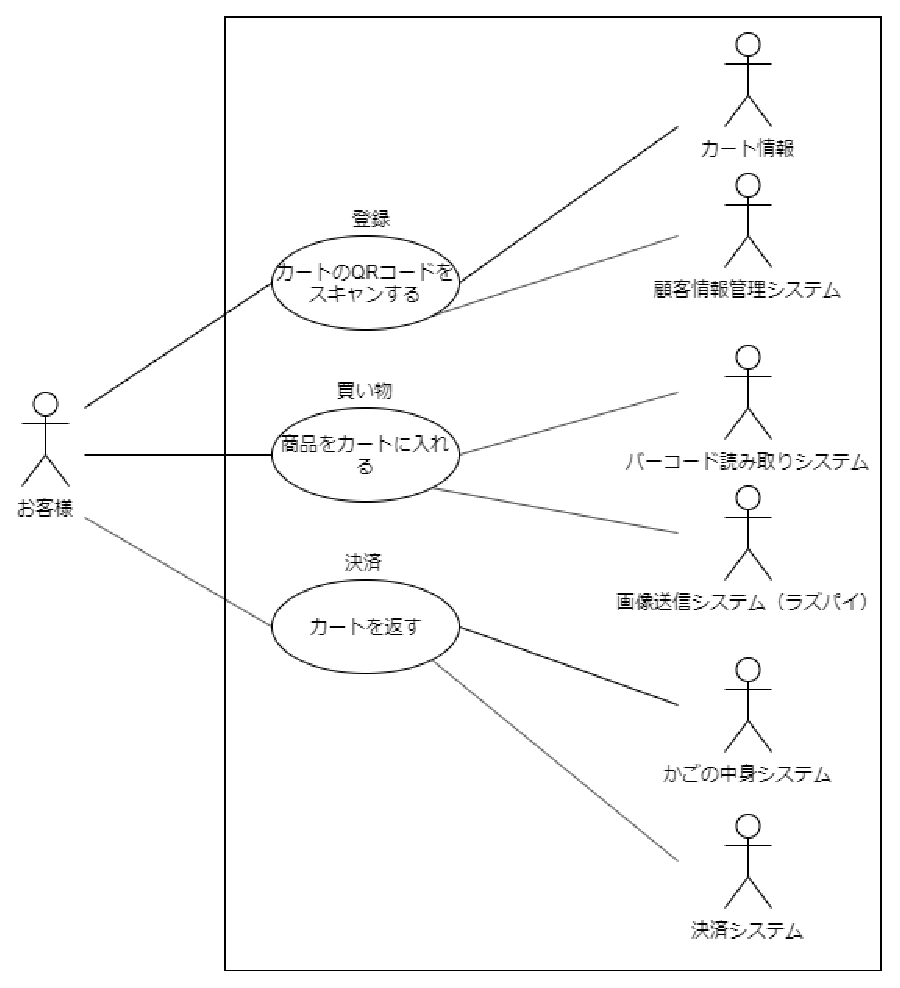
\includegraphics[width = 9cm]{./picture/usecase_qr.eps}
\caption{QRコードを用いたシステムのユースケース図}
\label{usecase_qr}
\end{figure}

図\ref{usecase_qr}はQRコードを用いた商品識別システムのユースケース図である.図\ref{usecase_qr}においては,まずQRコードを使用しカートもしくはカゴにQRコードを印刷したものを貼りつけ,それを入店時顧客が携帯電話等で読み取り,カゴ情報を顧客情報を結びつける.退店時は出口ゲートに設置したWebカメラでカートもしくはカゴのQRコードを読み取り,カゴ情報と顧客情報を管理する.


\begin{figure}[htbp]
\centering
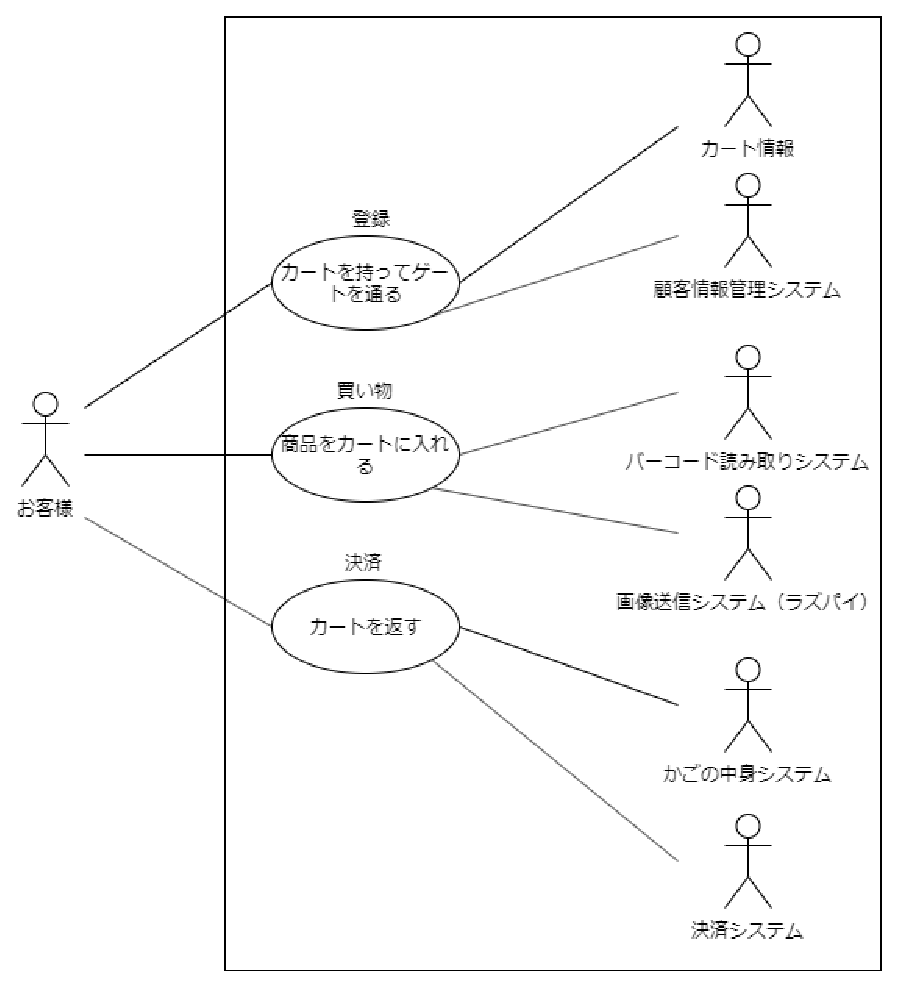
\includegraphics[width = 9cm]{./picture/usecase_ic.eps}
\caption{ICタグを用いたシステムのユースケース図}
\label{usecase_ic}
\end{figure}

図\ref{usecase_ic}はICタグを用いた商品識別システムのユースケース図である.図\ref{usecase_ic}においては,カートもしくはカゴにICタグを取り付け,入退店時にリーダーを設置したゲートを通ることで,カゴ情報と顧客情報を管理する.

%以下は3-2もしくは3-3で評価しようかな(下記の記述移動可能性)

それぞれの入退店時の案について基本の評価軸を用い,下記の表\ref{test}で評価した.


\begin{table}[htb]
\begin{center}
\caption{値段表}
\begin{tabular}{|l||c|c|c|} \hline
案 & コスト & 導入の容易さ & 簡単さ \\ \hline \hline
QRコード & 〇 & 〇 & × \\
ICタグ & × & △ & 〇 \\ \hline
\end{tabular}
\label{test}
  \end{center}
\end{table}


%具体的なカメラの台数やICタグの価格等を下記へ
評価した結果,よりQRコードを用いる案のほうがコストの面で優れている.しかしながら,簡単さという基準においては,携帯電話のカメラを起動して読み込む動作を顧客が行わなければならない点からQRコードを用いる案はあまり優れていないといえる.要求分析の段階ではどちらの案がよいかはかりかねたため,基本設計・詳細設計までそれぞれの案について設計した.